\documentclass[11pt]{article}
%\usepackage[T1]{fontenc}
%\usepackage[latin9]{inputenc}
\usepackage[margin=1in]{geometry}
\usepackage{csquotes}
\usepackage{xcolor}

% To compile in Times New Roman, use the following two lines.
% You'll need to compile with xelatex or lualatex.
% If you don't have these compilers, you can outcomment these two lines,
% but it won't be in Times New Roman.
\usepackage{fontspec}
\setmainfont{Times New Roman}

\usepackage{sectsty} % to get the section headings to be smaller
\usepackage{natbib}
\usepackage{bbm}
\usepackage{bm}
\usepackage{amsmath,amssymb,amsthm,mathtools}
\usepackage{caption}
\usepackage{algorithmic}
%\usepackage{authblk} % if you are using texlive on macports, install texlive-latex-extra to get this

% Uses the sectsty package to make section headings smaller.
\sectionfont{\fontsize{12}{15}\selectfont}
\subsectionfont{\fontsize{12}{15}\selectfont}

\newcommand{\Prob}{\mathbb{P}}
\newcommand{\E}{\mathbb{E}}
\newcommand{\EI}{\mathrm{EI}}
\newcommand{\Dir}{\mathrm{Dirichlet}}
\newcommand{\PI}{\text{PI}}
\newcommand{\mb}{\mathbf}
\newtheorem{Algorithm}{Algorithm}
\newtheorem{theorem}{Theorem}
\newtheorem{lemma}{Lemma}
\newtheorem{proposition}{Proposition}
\newtheorem{remark}{Remark}

\newcommand{\pfcomment}[1]{{\color{blue} PF: #1}}

\begin{document}

\title{Supplemental Information for \enquote{Peptide Optimization by Optimal Learning: 
Identification and refinement of peptides for reversible chemoenzymatic labeling}}
\maketitle
\tableofcontents
\newpage
\part{Supplementary Figures}
\part{Supplementary Methods}
\section{POOL Methodology}

We first introduce some mathematical notation that will allow precise discussion of the POOL methodology. Let $E$ be the set of peptides under consideration.
In our application, the set $E$ will be the set of peptides of length less than 38 amino acids.
For any peptide sequence $e \in E$, let $y(e) \in \{0, 1\}$ be a binary label indicating whether
peptide $e$ is active.  We suppose that this label can be observed directly through experiment, but is otherwise unknown {\it a priori}.
In our application, we consider several definitions of $y(e)$, depending on what kind of activity we are searching for:
\begin{itemize}
\item When searching for peptides with Sfp-specific activity, we let $y(e)$ be $1$ if the peptide is a substrate for both Sfp and AcpH, but is not a substrate for AcpS.  We call this an \enquote{Sfp-specific hit}.
\item When searching for peptides with AcpS-specific activity, we let $y(e)$ be $1$ if the peptide is a substrate for both AcpS and AcpH, but is not a substrate for Sfp.  We call this an \enquote{AcpS-specific hit}.
\end{itemize}

We further suppose that we are looking for active peptides that additionally have some
favored property, and the measure of favorability (for active peptides) can be
determined by a fitness function $f(e)$, which we suppose can be observed directly for all peptides without requiring a physical experiment. In our application, the fitness is negative one times the length of the peptide.  The negative one is present because we will want fitness to be large, but we want the length to be small.

Our goal is find a peptide $e\in E$ for which $y(e)=1$ and for which $f(e)$ is as large as possible.  We can write this problem as,
\begin{equation}
  \underset{e \in E, y(e) = 1}{\arg\max} \, f(e).
  \label{eq:general problem}
\end{equation}

% <<<<<<< HEAD
However, we cannot solve this problem directly because $y(e)$ has only been observed for those peptides on which we have performed an experiment, which is typically only a small fraction of the total number of peptides in $E$.  For example, in our application, $E$ contains more than $2 \times 10^{49}$ peptides, and we could only evaluate approximately $2500$ sequences, which is a tiny fraction of $E$.

Typically, we would have a budget that would allow us to evaluate $y(e)$ for only $k$ peptides, where $k$ is much smaller than $|E|$.  
In our application, $k$ is roughly $500$.
We might also have available to us $y(e)$ for some small number of previously evaluated peptides, 
\pfcomment{to be filled in.}


The question that we consider is how to use a limited experimental budget that allows us to evaluate $y(e)$ for some number $k$ of peptides $e$ in $E$, so as to best support solving \eqref{eq:general problem}.

We discuss our approach in the following sections: \ref{sec:existing approaches} reviews existing approaches, and points out the their existing problem;\ref{sec:stat model} describes the machine learning model we built for predicting $y(e)$; \ref{sec:prob improvement} shows our approach for solving \eqref{eq:general problem}; \ref{sec:contrast with predict-then-optimize} compares our approach to existing approaches, and discusses the advantages of our approach; \ref{sec:greedy algorithm}
provides an approximation algorithm for solving \eqref{eq:opt PI}, which is the core in our approach, and shows the approximation algorithm has performance guarantee in finding optimal value; \ref{sec:generality} discusses the generality of our proposed optimization method, which is compatible with a broad class of machine learning models while the performance guarantee still holds; \ref{sec:extension} discusses a possible extension to handle the search for peptides with multiple
types of activities; \ref{sec:application} shows results of using our approach in a real application.


\subsection{Existing Approaches} \label{sec:existing approaches}

We will contrast POOL with the existing way in which statistically-based predictions are used in the discovery of peptides, small molecules, and in other molecular discovery applications.
We focus on situations in which activity $y(e)$ is binary. In existing approaches, one would first collects some training data, in the form of peptide/activity pairs $(e,y(e))$, and train a machine learning classifier to make predictions $\hat{y}(e)$ of $y(e)$.  The classifier might be a naive Bayes classifier like the one that we use in Section~\ref{sec:stat model}, or some other classifier, e.g., a support vector machine \pfcomment{cite}, a random forest \pfcomment{cite}, or a neural network\pfcomment{cite}.
Depending on the classifier, the prediction may be binary, $\hat{y}(e) \in \{0,1\}$, or may be a real-valued score, $\hat{y}(e) \in [0,1]$ indicating a level of confidence, with values close to $0$ or $1$ indicating a high level of confidence, and values close to $1/2$ indicating a high level of uncertainty.  \pfcomment{Say something about the joint probability.}

For applications in which our goal is \eqref{eq:general problem}, and 

these predictions might be used in a variety of different ways.  The first would be to assume that the predictions are correct and then to sort those 


% \enquote{predict-then-optimize} approach, which is used by \pfcomment{Jialei, can you add some cites}, and which we believe to be the predominant way in which machine learning is used in the search for molecules with desirable properties.  


The predict-then-optimize approach assumes that the predictions $\hat{y}(e)$ are correct, and then solves, or approximately solves, the optimization problem 
\begin{equation*}
  \underset{e \in E, \hat{y}(e) = 1}{\arg\max} \, f(e).
  \label{}
\end{equation*}
It then recommends 


\begin{equation*}
  \underset{e \in E, f(e) \ge b}{\arg\max} \, P(y(e)=1)
  \label{}
\end{equation*}


While this approach works well when the predictions are highly accurate, we argue below in Section~\ref{sec:contrast with predict-then-optimize} that this approach is unnecessarily brittle to inaccuracies in predictions due to a lack of diversity that may appear in the set of peptides , and that peptide optimization with machine learning (POOL) provides more robust performance.


\subsection{Bayesian Machine Learning Model} \label{sec:stat model}

To predict whether a peptide is active or not, we develop a Naive Bayes classifier under Bayesian framework, which combines Naive Bayes and a prior distribution over unknown parameters encoding prior knowledge. This model provides the joint probability distribution over $y(e): e \in E$, which is needed to calculate $\PI(S)$. Suppose we can use a $J$-dimensional feature vector to represent a peptide, written as $\bm{x} = (x_1, \ldots, x_J)$, and the projection of $E$ to the feature space is $\mathcal{X}$, then the prediction problem is to calculate $\Prob (Y = y \mid \bm{X} = \bm{x})$, where $Y$ is random variable $\in \{0, 1\}$,
and $\bm{X} \in \mathcal{X}$ is random vector. Use Bayes' theorem, we have
\begin{equation}
  \Prob(Y = y \mid \bm{X} = \bm{x}) = \frac{\Prob(\bm{X} = \bm{x} \mid Y = y) \Prob(Y = y)}{\sum_{y' \in \{0, 1\}} \Prob(\bm{X}= \bm{x} \mid Y = y') \Prob(Y = y')}.
  \label{eq:NB_1}
\end{equation}
The Naive Bayes classifier assumes that the features are conditionally independent given $y$, then we can write \eqref{eq:NB_1} as 
\begin{equation}
  \Prob(Y = y \mid \bm{X} = \bm{x}) = \frac{\prod_{j = 1}^J \Prob(X_j = x_j \mid Y = y) \Prob(Y = y)}{\sum_{y' \in \{0, 1\}} \prod_{j = 1}^J \Prob(X_j = x_j \mid Y = y') \Prob(Y = y')}.
  \label{eq:NB_2}
\end{equation}
If we know $\Prob(X_j = x_j \mid Y = y)$ and $\Prob(Y = y)$, we can use \eqref{eq:NB_2} to calculate $\Prob(Y = y \mid \bm{X} = \bm{x})$ for any $\bm{x} \in \mathcal{X}$. Now the learning problem simply becomes estimating $\Prob(X_j = x_j \mid Y = y)$ and $\Prob(Y = y)$. We further assume $\Prob(X_j = x_j \mid Y = y)$ obeys categorical distribution with unknown parameters $\bm{\theta}^{y, j} = (\theta^{y, j}_1, \ldots, \theta^{y, j}_{K_j})$, that means $X_j$ has finite number of discrete values to choose from, and the probability of choosing each is determined by the parameters $\bm{\theta}^{y, j}$, written as $X_j \in \{1, \ldots, K_j\}$ and $\Prob(X_j = x_j \mid Y = y) = \theta^{y, j}_{x_j}$. Then \eqref{eq:NB_2} becomes
\begin{equation}
  \Prob (Y = y \mid \bm{X} = \bm{x}) = \frac{\Prob(Y = y) \prod_{j=1}^J \theta^{y, j}_{x_j}}
  {\Prob(Y = 1) \prod_{j=1}^J \theta^{1,j}_{x_j} + \Prob(Y = 0) \prod_{j=1}^J \theta^{0,j}_{x_j}}.
  \label{eq:NB_3}
\end{equation}
Since $\bm{\theta}^{y, j}$ are unknown, we use Bayesian inference to estimate them. We put Dirichlet prior distribution over $\bm{\theta}^{y, j}$, that is, $\bm{\theta}^{y, j} \sim Dirichlet(\bm{\alpha}^{y, j})$, where $\bm{\alpha}^{y, j}$ are parameters chosen initially to specify the prior distribution. We know the posterior distribution of $\bm{\theta}^{y, j}$ given training data $\{(\bm{x}^1, y^1), \ldots, (\bm{x}^N, y^N)\}$ is also a Dirichlet distribution, with new parameters $\overset{\sim}{\alpha}^{y, j}_k = \alpha^{y, j} + \sum_{n=1}^N \mathbbm{1}_{\{y^n = y, x^n_j = k\}}$, for $k = \{1, \ldots, K_j\}$. Now we can estimate $\Prob(Y = y \mid \bm{X} = \bm{x})$ using $\bm{\theta}^{y, j}$ drawn from their posterior distribution and \eqref{eq:NB_3}, if $\Prob(Y = 1)$ and $\bm{\alpha}^{y, j}$ are known, which can be estimated using cross validation. Here concludes the machine learning model we proposed and we will discuss the performance of this model in our application in \ref{sec:application}.

\subsection{Probability of Improvement} \label{sec:prob improvement} 
Many prediction methods, including all Bayesian prediction methods, provide a joint probability distribution over $y(e): e \in E$, which encodes prediction uncertainty. In our optimal learning approach, we use this joint probability distribution to define an auxiliary function, called probability of improvement, which quantifies the probability that a set of peptides $S$, if tested, will reveal an active peptide whose fitness $f(e)$ improves on some benchmark value $b$, which is typically the best $f(e)$ of active peptides observed in the past. We define this probability of improvement, $\PI(S)$, to be
\begin{equation}
  \PI(S) = \Prob \left( \max_{e \in S, y(e)=1} f(e) > b \right).
  \label{}
\end{equation}
To ensure consistency, we define $\max$ over an empty set is $-\infty$. We find $S$ by solving
\begin{equation}
  \underset{S \subseteq E, |S| \leq M}{\arg\max} \PI(S),
  \label{eq:opt PI}
\end{equation}
where $M$ is the number of peptides that can be tested simultaneously in a single round of experiment. After we find the set $S$ and tested the peptides in it, we use the results along with previously tested peptides as training data, and find a new set $S$ for the next round of experiment. We repeat this process until we find enough favored active peptides or resource is exhausted. We demonstrate in an application of finding reversible chemoenzymatic labeling peptides that this approach performs better than existing approaches. This use of the probability of improvement builds on previous work in engineering for global optimization of time-consuming computer codes [add cites], and also on value-of-information and optimal learning methods in that same application area [add cites].

\subsection{Contrast with predict-then-optimize method} \label{sec:contrast with predict-then-optimize}
While the predict-then-optimize approach works well when the predictions by machine learning model are highly accurate, due to the nature of similar sequences have similar prediction value from machine learning model, the recommended sequences to test from this approach are generally very similar to each other, i.e., lack of diversity. When the predictions are not accurate, especially in the case of small training dataset, testing very similar sequences is risky, because if one sequence
turns out to be not a hit, then the other sequences are not likely to be a hit either. However, maximizing probability of improvement tends to give you more diversified sequences, and there is a simple reasoning behind this: suppose there are three peptides, $A, B$ and $C$ and we only want to pick two of them for test; A and B are very similar to each other, and their predicted probability being a hit is $\Prob (A \text{ is a hit}) = \Prob (B \text{ is a hit}) = 0.9$, while $C$ is
quite different from $A$ or $B$, and $C$ has a lower predicted probability being a hit,
say $\Prob (C \text{ is a hit}) = 0.8$. Predict-then-optimize approach will pick $A$ anad $B$ because they both have higher predicted probability being a hit, however, you will see choosing $A$ and $B$ does not give you the highest probability of improvement through calculation. To simplify the demonstration, let's assume correlation between $A$ being a hit and $B$ being a hit is $1$, both $A$ being a hit and $B$ being a hit are independent from $C$ being a hit, and $f(A), f(B), f(C)$ are all greater than
$b$, then $\PI (\{A, B\}) = \Prob (A \text{ is a hit}, B \text{ is a hit}) + \Prob (A \text{ is a hit}, B \text{ is not a hit}) + \Prob (A \text{ is not a hit}, B \text{ is a hit}) = 0.9 + 0 + 0 = 0.9$, and $\PI (\{A, C\}) = \Prob (A \text{ is a hit}, C \text{ is a hit}) + \Prob (A \text{ is a hit}, C \text{ is not a hit}) + \Prob (A \text{ is not a hit}, C \text{ is a hit}) = 0.9 \times 0.8 + 0.9 \times 0.2 + 0.1 \times 0.8 = 0.98$. Thus maximing probability will choose either $A$ and $C$ or $B$ and $C$, and this
more diversified than the recommendations given by predict-then-optimize approach. Now suppose we performed test, and turns out $A$ is not a hit, then $B$ is not likely to be a hit either, while $C$ is different than $A$ and thus there is still good chance that $C$ is a hit. Therefore, maximizing probability of improvement has better chance to find hits even the predictions by machine learning model is not accurate enough.

\subsection{Greedy Algorithm} \label{sec:greedy algorithm}
Directly solving \eqref{eq:opt PI} is impractical, because computational cost for $\PI(S)$
grows exponentially with $M$, not to mention the optimization problem is even harder than
computing the objective function, considering the number of sets $S$ satisfying $|S| \leq M$
also grows exponentially with $M$. Instead we employ approximation methods, and the approximation
method we employ is a greedy algorithm, which starts with $S = \emptyset$, and then adds
peptides one-by-one, each time choosing the one that will increase the probability of 
improvement by the greatest amount, that is, solving 
\begin{equation}
  \underset{e \in E \backslash S}{\mathrm{arg}\max} \,\PI (S \cup \{e\}),
  \label{eq:greedy}
\end{equation}
until $|S| = M$. This algorithm has much smaller computational challenge, for two reasons:
first, the size of search space reduces from $|E|^M$ to $|E| \times M$; second, as will be pointed
out in Proposition \ref{prop:reduced form}, solving \eqref{eq:greedy} does not require computing $\PI$.
Before going into detail of solving \eqref{eq:greedy}, I like to use the following section
to show that this greedy algorithm has theoretic performance guarantee, and this result holds
for any machine learning model that can compute probability of improvement.

\subsubsection{Performance Guarantee for the Greedy Algorithm} \label{sec:lower bound}
The main result is stated in the following theorem:
\begin{theorem} 
  The greedy algorithm always produces a solution whose probability of improvement is at 
  least $1-[(M-1)/M]^M \geq 1 - 1 / e$ times the optimal objective
  value of \eqref{eq:opt PI}.
\end{theorem}
To prove the theorem, we use the following two lemmas:
\begin{lemma} \citep{nemhauser1978analysis}
  If $F(S)$ is submodular, nondecreasing and $F(\emptyset)=0$, the greedy heuristic always 
  produces a solution whose value is at least $1-[(M-1)/M]^M$ times the optimal value, where 
  $|S| \leq M$. This bound can be achieved for each $M$ and has a limiting value of $1-1/e$, 
  where $e$ is the base of the natural logarithm.
\end{lemma}

\begin{lemma} 
  Probability of improvement $\PI(S)$ is submodular, nondecreasing and $\PI(\emptyset)=0$.
\end{lemma}
\begin{proof}
Let $f^*(S) = \max_{e \in S, y(e)=1} f(e)$. First we show $\PI(\emptyset) = 0$.
\begin{equation*}
  \PI(\emptyset) = \Prob(f^*(\emptyset) > b) = \Prob(-\infty > b)=0.
\end{equation*}

To show $\PI(S)$ is nondecreasing, let $A \subseteq B \subseteq E$ where $E$ is a finite set, then
\begin{equation*}
\begin{split}
\PI(B) &= \Prob(f^*(B) > b) \\
       &= \Prob(f^*(B) > b \mid f^*(A) \leq b) \Prob(f^*(A) \leq b) + \Prob(f^*(B) > b \mid f^*(A) > b) \Prob(f^*(A) > b) \\
       &= \Prob(f^*(B) > b \mid f^*(A) \leq b) \Prob(f^*(A) \leq b) + \Prob(f^*(A) > b) \\
       &\leq \Prob(f^*(A) > b) \\
       &= \PI(A)
\end{split}
\end{equation*}

Lastly, we want to show $\PI(S)$ is submodular. For $e \in E\backslash B$,
\begin{equation*}
  \begin{split}
    &\PI(A \cup \{e\}) - \PI(A) \\
    &= \Prob(f^*(A \cup \{e\}) > b) - \Prob(f^*(A) > b) \\
    &= \Prob(f^*(A \cup \{e\}) > b \mid f^*(A) > b) \Prob(f^*(A) > b) \\
    &\quad + \Prob(f^*(A \cup \{e\}) > b \mid f^*(A) \leq b)
    \Prob(f^*(A) \leq b) - \Prob(f^*(A) > b) \\
    &= \Prob(f^*(A \cup \{e\}) > b \mid f^*(A)\leq b) \Prob(f^*(A)\leq b) \\
    &= \Prob(f(e) > b, y(e) = 1 \mid f^*(A) \leq b) \Prob(f^*(A) \leq b) \\
    &= \Prob(f(e) > b, y(e) = 1, f^*(A) \leq b)
  \end{split}
\end{equation*}
Using similar argument,
\begin{equation*}
\begin{split}
&\PI(B \cup \{e\}) - \PI(B) \\
&= \Prob(f(e)<b, y(e)=1,f^*(B)\geq b) \\
&= \Prob(f(e)<b, y(e)=1,f^*(A)\geq b, f^*(B\backslash A) \geq b )
\end{split}
\end{equation*}
Therefore, $\PI(A \cup \{e\}) - \PI(A) \geq \PI(B \cup \{e\}) - \PI(B)$, thus $\PI(S)$ is submodular. \qedhere
\end{proof}

Lemma 1 is a result from the analysis of greedy heuristic in combinatorial optimization by 
Nemhauser, who provides lower bound of greedy heuristic given that objective function 
satisfies certain conditions. Lemma 2 shows that $\PI(S)$ satisfies condition stated in 
Lemma 1, therefore, theorem 1 holds. Note that the proof does not rely on a particular machine
learning model.

\subsubsection{Reduced Form of Greedy Algorithm} \label{sec:reduced form}
Since $\PI(S)$ is expensive to compute when $|S|$ is large, in Proposition 
\ref{prop:reduced form}, we show that \eqref{eq:greedy} can be written into a
form in which the objective function can be easily computed. The result
holds for any machine learning model that can compute the objective in
\eqref{eq:reduced form}.
\begin{proposition} \label{prop:reduced form}
  Solving \eqref{eq:greedy} is equivalent to solving
  \begin{equation}
    \underset{e \in E \backslash S, f(e) > b}{\mathrm{arg}\max} \, \Prob (y(e)=1 \mid y(e') = 0, \forall e' \in S).
    \label{eq:reduced form}
  \end{equation}
\end{proposition}
\begin{proof}
  \begin{equation*}
    \begin{split}
      &\PI(S \cup \{e\}) = \Prob(f^*(S\cup \{e\}) > b)\\
      &= \Prob(f^*(S) > b) + \Prob(f^*(S)\leq b) \Prob(f(e) > b, y(e) = 1 \mid f^*(S)\leq b),
    \end{split}
  \end{equation*}
  so \eqref{eq:greedy} becomes
  \begin{equation} \label{eq:PI1} 
    \underset{e \in E \backslash S}{\max} \, \PI(S \cup \{e\}) = \underset{e \in E \backslash S}{\max} \, \Prob(f(e) > b, y(e)=1 \mid f^*(S)\leq b).
  \end{equation}
  Note that when $f(e) \leq b$, $\Prob(f(e) > b, y(e) = 1 \mid f^*(S)\leq b) = 0$, thus our algorithm will always propose $e$ such that $f(e) > b$. Therefore, it is reasonable to assume that $f(x) > b$ for $\forall x \in S$, and $f^*(S)\leq b$ is equivalent to $y(e') = 0$ for $\forall e' \in S$. Now we can write \eqref{eq:PI1} as 
  \begin{equation*}
    \underset{e \in E \backslash S, f(e) > b}{\max} \, \Prob (y(e) = 1 \mid y(e') = 0, \forall e' \in S). 
  \end{equation*}
\end{proof}

\subsubsection{Intuition Behind Reduced Form}
From Proposition \ref{prop:reduced form}, we have seen that the greedy algorithm is equivalent to an algorithm that chooses each new peptide to test by supposing that all previously added peptides did not produce the desired result, and adding this supposition as additional \enquote{training data} to provide a new estimate of peptide activity. Through this lens, we see that the optimal learning approach explicitly provides diversity in its search for high-quality peptides, which is in consistant with the conclusion in \ref{sec:contrast with predict-then-optimize}.

\subsubsection{Solving Greedy Step with MINLP} \label{sec: MINLP approach}
Under the Naive Bayes model proposed in section \ref{sec:stat model}, 
we can formulate \eqref{eq:reduced form} as an instance of Mixed-Integer 
Nonlinear Program (MINLP), and then we can use any off-the-shelf MINLP 
solver to solve the greedy step. First we write \eqref{eq:NB_3} as
\begin{equation}
  \Prob (Y = 1 \mid \bm{x}) = \frac{\prod_{j=1}^J \eta^j_{x_j}}
  {\prod_{j=1}^J \eta^j_{x_j} + \frac{\Prob(Y = 0)}{\Prob(Y = 1)}},
  \label{eq:MINLP_2}
\end{equation}
where
\begin{equation*}
  \eta^j_{x_j} = \frac{\theta^{1,j}_{x_j}}{\theta^{0,j}_{x_j}}
  \text{\,\,\,for $\forall j \in \{1,\ldots,J\}$}. 
\end{equation*}
Then we can write \eqref{eq:reduced form} as
\begin{equation}
  \underset{e \in E \backslash S, f(e) > b}{\mathrm{arg}\max} \, \frac{\prod_{j = 1}^J \eta^j_{x_j}}{\prod_{j = 1}^J \eta^j_{x_j} + \frac{\Prob(Y = 0)}{\Prob(Y = 1)}},
  \label{eq:MINLP_3}
\end{equation}
where $\bm{x}$ is feature vector of peptide $e$, and
\begin{equation*}
  \eta^j_{x_j} = \frac{\Prob(X_j = x_j \mid Y = 1, y(e') = 0, \forall e' \in S)}
  {\Prob(X_j = x_j \mid Y = 0, y(e') = 0, \forall e' \in S)}.
\end{equation*}
We can write \eqref{eq:MINLP_3} as a Mixed-Integer Nonlinear Program,
\begin{equation}
  \begin{split}
    \max \quad &\frac{\prod_{j=1}^J \sum_{k=1}^{K_j} z^j_k \eta^j_k}
    {\prod_{j=1}^J \sum_{k=1}^{K_j} z^j_k \eta^j_k + \frac{\Prob(Y = 0)}{\Prob(Y = 1)}} \\
    \text{s.t} \quad &z^j_k \in \{0,1\}\\
    &\sum_{k=1}^{K_j} z^j_k = 1, \,\, \forall j \in \{1, \ldots, J\}
  \end{split}
  \label{eq:MINLP_4}
\end{equation}
where
\begin{equation*}
z^j_k = \begin{dcases}
        1 & \text{if $x_j = k$}\\
        0 & \text{else}.
\end{dcases}
\end{equation*}
The constraints in \eqref{eq:MINLP_4} do not account for $f(e) > b$, because it depends on
the $f(\cdot)$ to design the corresponding constraint, and for now we assume this
constraint is met. Since $\eta^j_k$s are unknown, we can sample $\eta^j_k$s from their posterior 
distribution, which can be obtained from the machine learning model in \ref{sec:stat model},
and solve \eqref{eq:MINLP_4} for each instance of $\eta^j_k$, then we pick
the solution with highest objective in \eqref{eq:reduced form}. We summarize 
the algorithm in the following:
\begin{Algorithm}(Probability of Improvement) \label{algo1}
\begin{algorithmic}[1]
  \REQUIRE Inputs $M, J, K_j, j = \{1, \ldots, J\}$, data set $\mathcal{D} = 
  \{(\bm{x}^1, y^1), \ldots, (\bm{x}^N, y^N)\}$ and parameters for the prior 
  distributions $\bm{\alpha}^{y, j}$.
  \STATE $S \leftarrow \emptyset $
  \STATE Calculate posterior distribution of $\bm{\theta}^{1, j} \sim 
  \text{Dirichlet} (\bm{\theta}^{1, j} \mid \{\bm{x}: \bm{x} \in \mathcal{D}, 
  y(\bm{x}) = 1\})$.
  \FOR{$m=1$ to $M$} 
    \STATE COUNT $\leftarrow 0$
    \STATE Calculate posterior distribution of $\bm{\theta}^{0, j} \sim 
    \text{Dirichlet} (\bm{\theta}^{0, j} \mid \{\bm{x}: \bm{x} \in \mathcal{D}, 
    y(\bm{x}) = 1\} \cup S)$.
    \FOR{$i=1$ to $I$}
      \STATE Sample $\bm{\theta}^{1, j}$ from $\text{Dirichlet} (\bm{\theta}^{1, j} 
      \mid \{\bm{x}: \bm{x} \in \mathcal{D}, y(\bm{x}) = 1\})$ and $\bm{\theta}^{0, j}$
      from $\text{Dirichlet} (\bm{\theta}^{0, j} \mid \{\bm{x}: \bm{x} \in \mathcal{D}, 
      y(\bm{x}) = 1\} \cup S)$.
      \STATE $\eta^j_k \leftarrow \frac{\theta^{1, j}_k}{\theta^{0, j}_k}$
      \STATE Solve MINLP in \eqref{eq:MINLP_4} to find $\bm{x}^i$ and the corresponding
      peptide sequence $e^i$.
    \ENDFOR
    \STATE $e^* \leftarrow \underset{e \in \{e^1, \ldots, e^I\}}
    {\arg \max} \Prob (y(e) = 1 \mid y(e') = 0, \forall e' \in S)$.
    \STATE $S \leftarrow (S, e^*)$.
  \ENDFOR
\end{algorithmic}
\end{Algorithm}

\subsubsection{Solving Greedy Step with MAP Estimation}
In our application of finding reversible labeling peptides, the dimension of search space is so high that solving MINLP as in \ref{sec: MINLP approach} is computationally challenging. We propose another simpler approach, that is, Maximum a Posteriori estimation, to solve \eqref{eq:NB_3}. While this approach does not provide as high quality solution as MINLP does, the computation is very quick and easy. 

\subsection{Generality of Approach} \label{sec:generality}
While we proposed a Naive Bayes model for prediction in \ref{sec:stat model}, the optimal learning approach that we proposed is rather general and applies to any machine learning model as long as it allows calculation of the objective in \eqref{eq:reduced form}, for example, you can easily plug in common machine learning classifiers like logistic regression, SVM with probabilistic output, etc. The result of performance guarantee of the greedy algorithm in ref{sec:lower bound} and the
reduced form of greedy algorithm in \ref{sec:reduced form} applies, too.

\subsection{Extension to Handle Search for Specific Activity} \label{sec:extension}
In our application of searching peptides with specific activity, we do not only obtain one label for each peptide that is tested, instead, we observe multiple labels and each is associated with reaction between the peptide and a specific enzyme, and we determine the final label from these observed labels. Mathematically, we can write it as, for peptide $e$, its label $y(e) = \prod_i y_i(e)$ and we observe $y_i(e)$. To utilize as much information as possible, instead of building Naive Bayes
classifier predicting $y(e)$ directly, we build separate Naive Bayes classifiers predicting each $y_i(e)$, and rewrite \eqref{eq:reduced form} as
\begin{equation*}
  \underset{e \in E \backslash S, f(e) > b}{\mathrm{arg}\max} \, \Prob (y_i(e)=1, \forall i \mid \prod_i y_i(e') = 0, \forall e' \in S).
  \label{}
\end{equation*}
The objective is hard to compute because the number of configurations of $y_i(e'), \forall e \in S$ that satisfy $\prod_i y_i(e') = 0$ grows exponentially with the size of $S$. We adopt a heuristic approach, which is to approximate the objective by
\begin{equation}
  \Prob (y_i(e)=1, \forall i \mid y_i(e'), \forall i, \forall e' \in S),
  \label{}
\end{equation}
and we choose $y_i(e')$ as long as they satisfy $\prod_i y_i(e') = 0, \forall e' \in S$.

\subsection{Application} \label{sec:application}
First we show this application is an instance of the more general problem discussed
at the beginning. The goal in this specific problem is to find short peptides that 
are labeled by specific PPTases and unlabeled by ACPH, thus we let $y(e) = 1$
if peptide $e$ has this property. Since we are looking for short peptides, let the
utility function $f(e)$ be negative the length of peptide $e$, and now the problem
is the same as \eqref{eq:general problem}.

\subsubsection{Performance of Machine Learning Model}
We use the machine learning model described in \ref{sec:stat model} to predict $y(e)$.
The feature vector for peptides is designed in the following: since the chemoenzymatic
reaction only happens at position containing Serine within the peptide, we are looking 
for the peptides containing exactly one Serine in the sequence. We use the position 
containing Serine as the origin, and each feature corresponds to a position, which is
counted from the origin towards C-terminus or N-terminus. For example, a sequence
X-X-X-S-X-X, where S represents Serine and X represents any amino acid in that
position, has features N1, N2, N3, C1, C2, and the correspondence in position is
N3-N2-N1-S-C1-C2. Each feature's value is determined by the amino acid residing in
the corresponding position. In this application, to reduce dimensionality of the 
feature space, we group the 20 standard amino acids into 8 classes according to
their similarity, and the feature values for the amino acids belonging to the 
same class are the same. The grouping detail is shown in [refer to reduced AA table].

After constructing the features, we train the model following the method outlined
in \ref{sec:stat model}. To validate our model, we use leave-one-out 
cross validation to plot receiver operating characteristic (ROC), which
is typically used to benchmark performance of binary classifiers.

\begin{figure}[hpt] 
\center
\begin{minipage}[b]{0.45\linewidth}
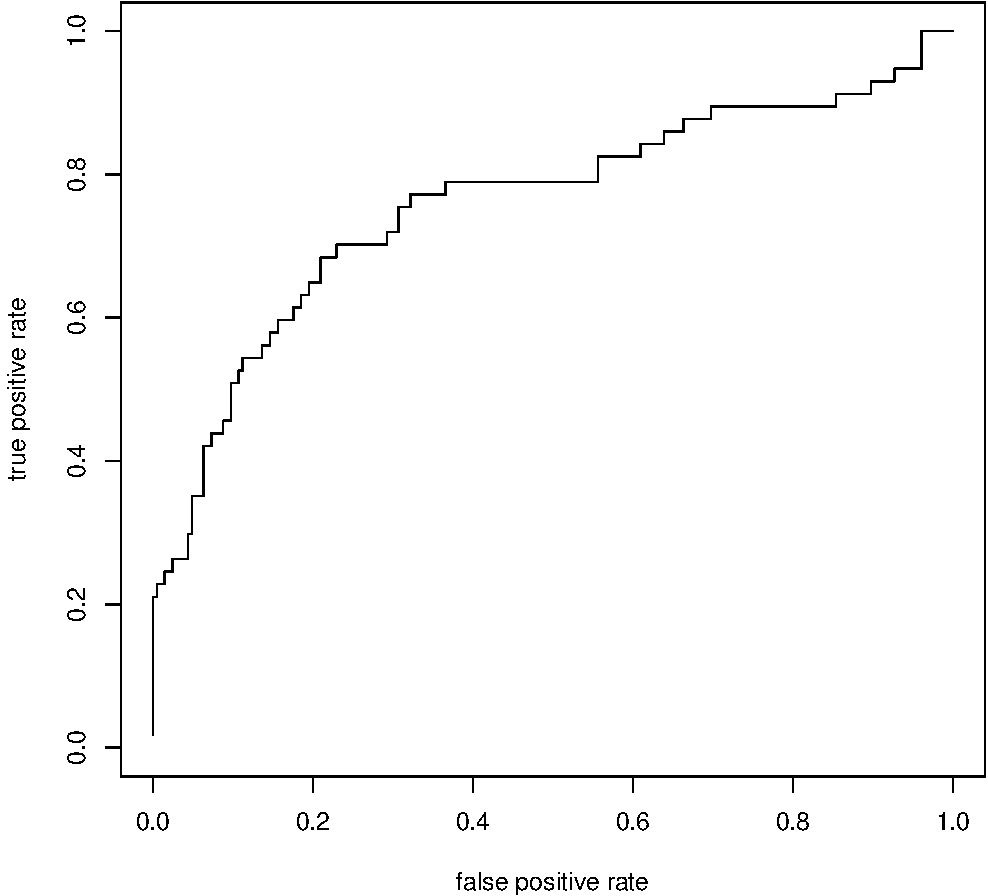
\includegraphics[width=\textwidth]{pic/ROC_DS1_1000_025.pdf}
\end{minipage}
\begin{minipage}[b]{0.45\linewidth}
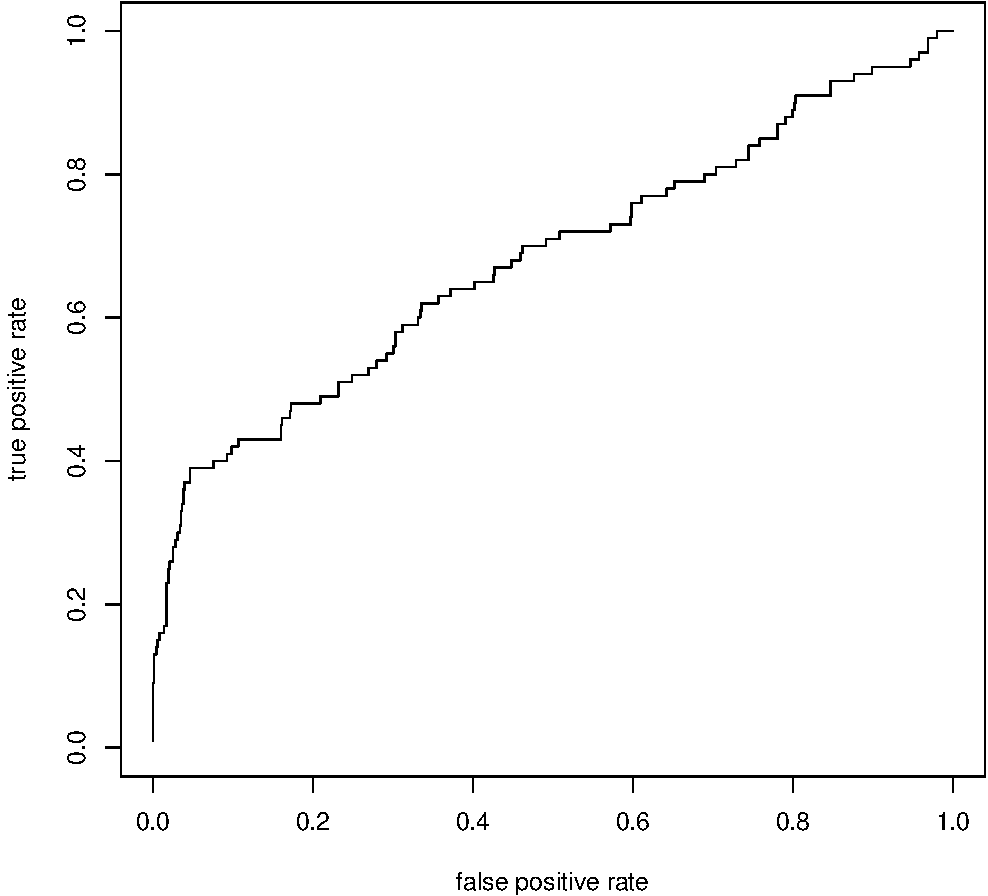
\includegraphics[width=\textwidth]{pic/ROC_DS2_1000_025.pdf}
\end{minipage}
\caption{ ROC curve using leave-one-out cross validation}
\label{fig:ROC}
\end{figure}


\subsubsection{Comparison of POOL v.s. other existing methods}
Describe setup of simulation for the benchmark plot?


\section{General materials and methods}
\section{Lead peptides with fluorophores}
\section{Sequence alignment of lead peptides}
\part{Supplementary Tables}

\bibliography{nature_SI}
\bibliographystyle{plainnat}
%%%%%%%%%%%%%%%%%
\end{document}
%%%%%%%%%%%%%%%%%
